\documentclass{standalone}
\usepackage{tikz}
\usetikzlibrary{patterns, positioning}
\usepackage[sfdefault]{ClearSans} %% option 'sfdefault' activates Clear Sans as the default text font
\usepackage[T1]{fontenc}

\begin{document}
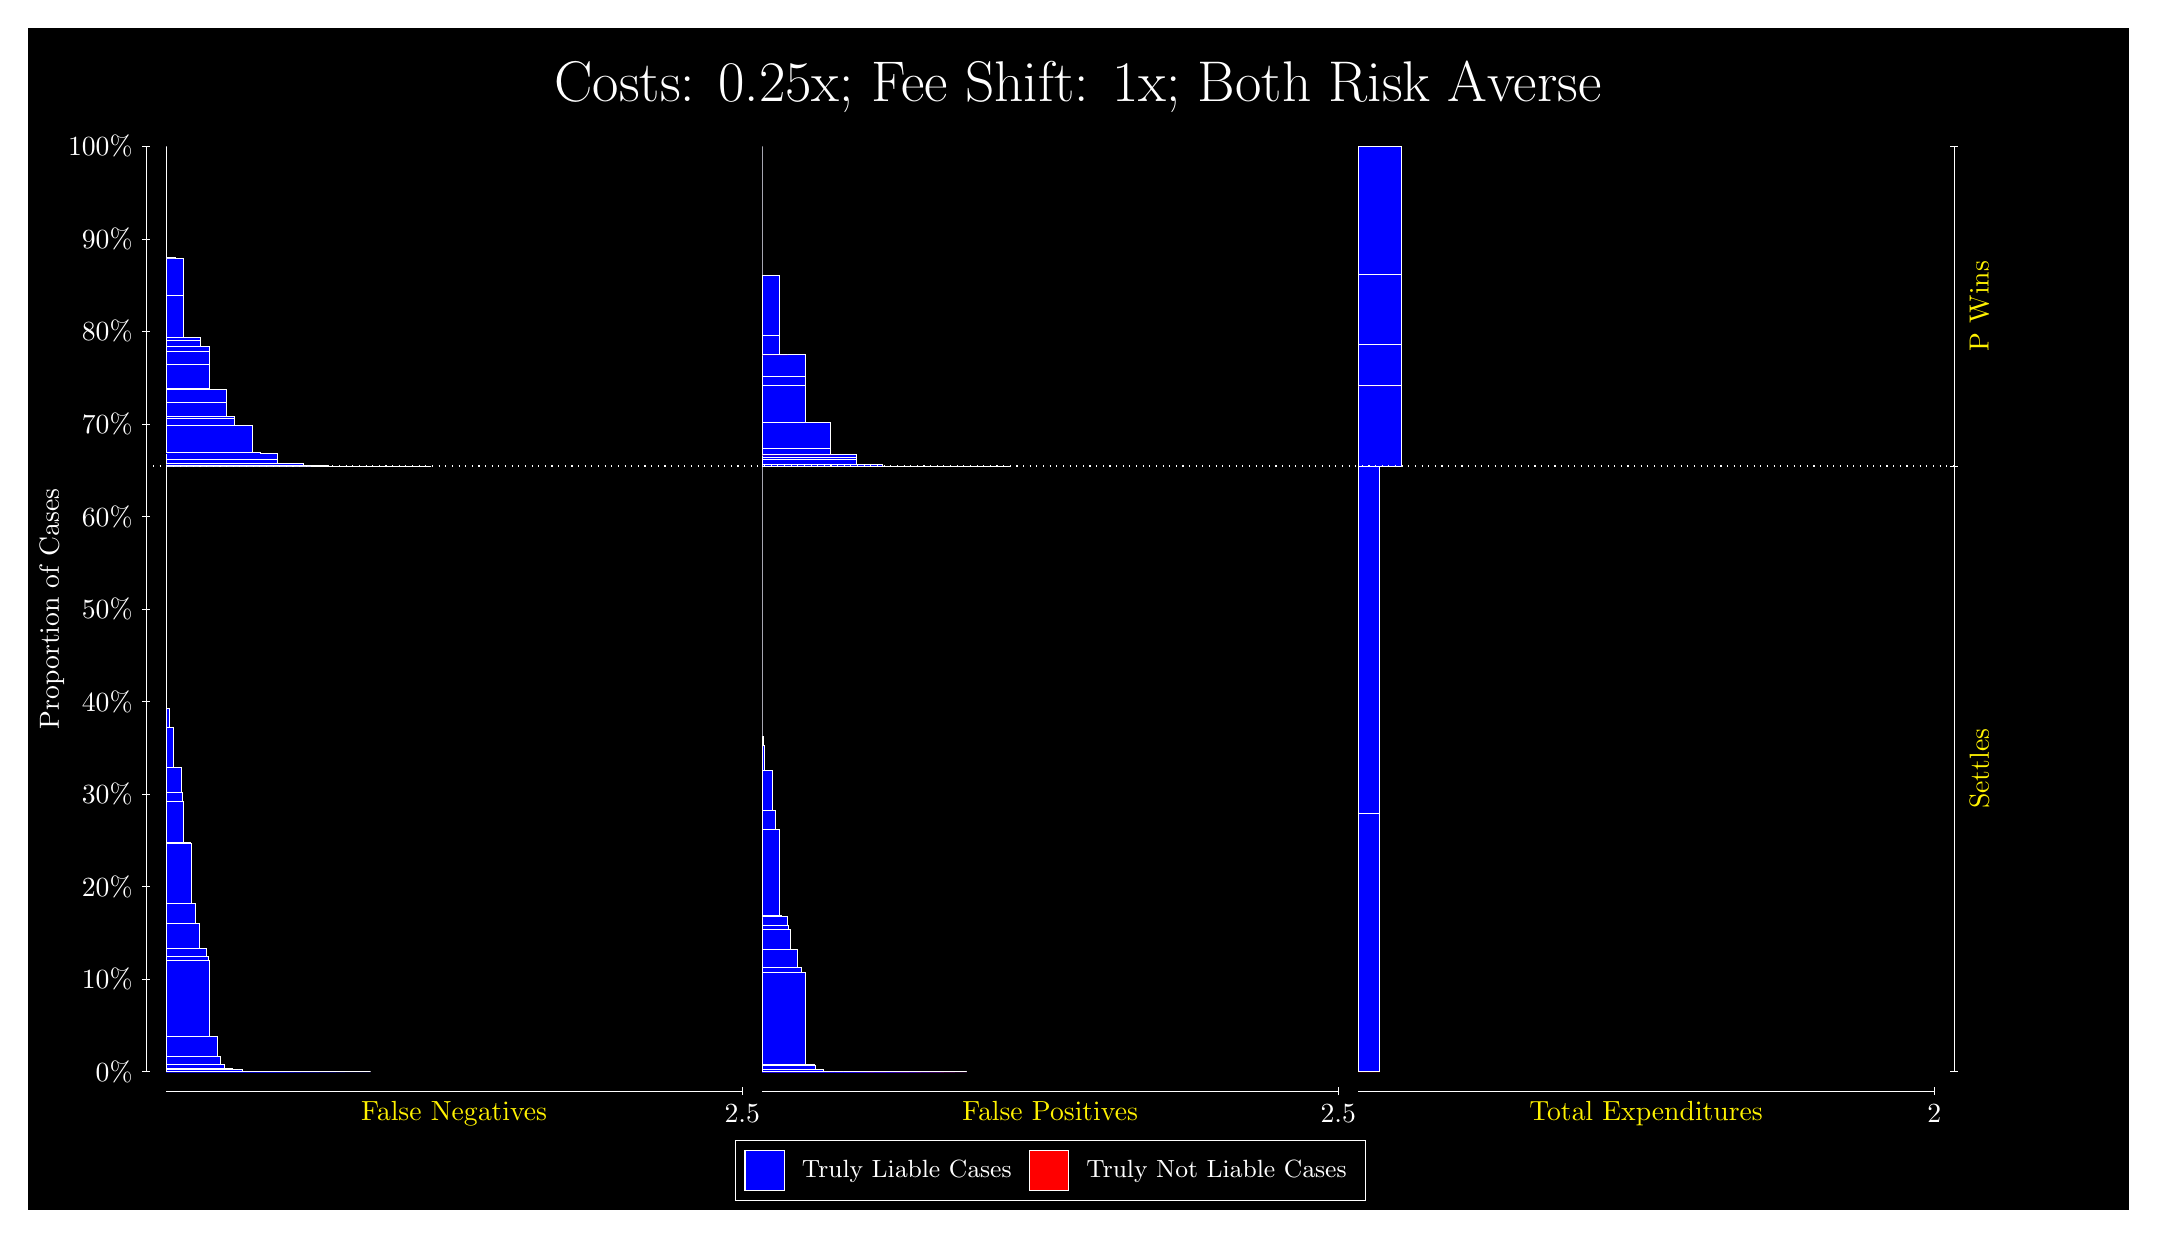
\begin{tikzpicture}
\draw[fill=black] (0,0) rectangle (26.667,15);
\draw[text=white] (0,13.5) rectangle (26.667,15) node[midway] {\huge Costs: 0.25x; Fee Shift: 1x; Both Risk Averse};
\draw[white, very thin] (1.5,1.75) -- (1.5,13.5);
\node[rotate=90, text=white, anchor=center] at (0.3, 7.625) {Proportion of Cases};
\draw[white, very thin] (1.45,1.75) -- (1.55,1.75);
\node[text=white, anchor=east] at (1.45, 1.75) {0\%};
\draw[white, very thin] (1.45,2.925) -- (1.55,2.925);
\node[text=white, anchor=east] at (1.45, 2.925) {10\%};
\draw[white, very thin] (1.45,4.1) -- (1.55,4.1);
\node[text=white, anchor=east] at (1.45, 4.1) {20\%};
\draw[white, very thin] (1.45,5.275) -- (1.55,5.275);
\node[text=white, anchor=east] at (1.45, 5.275) {30\%};
\draw[white, very thin] (1.45,6.45) -- (1.55,6.45);
\node[text=white, anchor=east] at (1.45, 6.45) {40\%};
\draw[white, very thin] (1.45,7.625) -- (1.55,7.625);
\node[text=white, anchor=east] at (1.45, 7.625) {50\%};
\draw[white, very thin] (1.45,8.8) -- (1.55,8.8);
\node[text=white, anchor=east] at (1.45, 8.8) {60\%};
\draw[white, very thin] (1.45,9.975) -- (1.55,9.975);
\node[text=white, anchor=east] at (1.45, 9.975) {70\%};
\draw[white, very thin] (1.45,11.15) -- (1.55,11.15);
\node[text=white, anchor=east] at (1.45, 11.15) {80\%};
\draw[white, very thin] (1.45,12.325) -- (1.55,12.325);
\node[text=white, anchor=east] at (1.45, 12.325) {90\%};
\draw[white, very thin] (1.45,13.5) -- (1.55,13.5);
\node[text=white, anchor=east] at (1.45, 13.5) {100\%};

\draw[white, very thin] (24.457,1.75) -- (24.457,13.5);
\draw[white, very thin] (24.407,1.75) -- (24.507,1.75);
\node[anchor=west] at (24.407, 1.75) {};
\draw[white, very thin] (24.407,9.4406) -- (24.507,9.4406);
\node[anchor=west] at (24.407, 9.4406) {};
\draw[white, very thin] (24.407,13.5) -- (24.507,13.5);
\node[anchor=west] at (24.407, 13.5) {};

\draw[white, very thin, fill=blue] (1.75,1.75) rectangle (4.3482,1.75);
\draw[white, very thin, fill=blue] (1.75,1.75) rectangle (4.0229,1.75);
\draw[white, very thin, fill=blue] (1.75,1.75) rectangle (3.9091,1.75);
\draw[white, very thin, fill=blue] (1.75,1.75) rectangle (3.6976,1.75);
\draw[white, very thin, fill=blue] (1.75,1.75) rectangle (3.5838,1.75);
\draw[white, very thin, fill=blue] (1.75,1.75) rectangle (3.4699,1.75);
\draw[white, very thin, fill=blue] (1.75,1.75) rectangle (3.3723,1.75);
\draw[white, very thin, fill=blue] (1.75,1.75) rectangle (3.3236,1.75);
\draw[white, very thin, fill=blue] (1.75,1.75) rectangle (3.2585,1.75);
\draw[white, very thin, fill=blue] (1.75,1.75) rectangle (3.1447,1.75);
\draw[white, very thin, fill=blue] (1.75,1.75) rectangle (3.0471,1.7505);
\draw[white, very thin, fill=blue] (1.75,1.7505) rectangle (3.0308,1.7505);
\draw[white, very thin, fill=blue] (1.75,1.7505) rectangle (2.9983,1.7505);
\draw[white, very thin, fill=blue] (1.75,1.7505) rectangle (2.9332,1.7507);
\draw[white, very thin, fill=blue] (1.75,1.7507) rectangle (2.8844,1.7507);
\draw[white, very thin, fill=blue] (1.75,1.7507) rectangle (2.8194,1.753);
\draw[white, very thin, fill=blue] (1.75,1.753) rectangle (2.7218,1.7772);
\draw[white, very thin, fill=blue] (1.75,1.7772) rectangle (2.7055,1.7773);
\draw[white, very thin, fill=blue] (1.75,1.7773) rectangle (2.673,1.7773);
\draw[white, very thin, fill=blue] (1.75,1.7773) rectangle (2.6079,1.7836);
\draw[white, very thin, fill=blue] (1.75,1.7836) rectangle (2.5917,1.7935);
\draw[white, very thin, fill=blue] (1.75,1.7935) rectangle (2.5591,1.7937);
\draw[white, very thin, fill=blue] (1.75,1.7937) rectangle (2.4941,1.8474);
\draw[white, very thin, fill=blue] (1.75,1.8474) rectangle (2.4453,1.95);
\draw[white, very thin, fill=blue] (1.75,1.95) rectangle (2.3965,2.2005);
\draw[white, very thin, fill=blue] (1.75,2.2005) rectangle (2.3802,2.2033);
\draw[white, very thin, fill=blue] (1.75,2.2033) rectangle (2.3477,2.2034);
\draw[white, very thin, fill=blue] (1.75,2.2034) rectangle (2.2989,3.1623);
\draw[white, very thin, fill=blue] (1.75,3.1623) rectangle (2.2827,3.2161);
\draw[white, very thin, fill=blue] (1.75,3.2161) rectangle (2.2664,3.3166);
\draw[white, very thin, fill=blue] (1.75,3.3166) rectangle (2.2339,3.3189);
\draw[white, very thin, fill=blue] (1.75,3.3189) rectangle (2.1688,3.6271);
\draw[white, very thin, fill=blue] (1.75,3.6271) rectangle (2.12,3.8869);
\draw[white, very thin, fill=blue] (1.75,3.8869) rectangle (2.0712,4.6427);
\draw[white, very thin, fill=blue] (1.75,4.6427) rectangle (2.055,4.6616);
\draw[white, very thin, fill=blue] (1.75,4.6616) rectangle (2.0224,4.6616);
\draw[white, very thin, fill=blue] (1.75,4.6616) rectangle (1.9736,5.1881);
\draw[white, very thin, fill=blue] (1.75,5.1881) rectangle (1.9574,5.2999);
\draw[white, very thin, fill=blue] (1.75,5.2999) rectangle (1.9411,5.6121);
\draw[white, very thin, fill=blue] (1.75,5.6121) rectangle (1.9086,5.6173);
\draw[white, very thin, fill=blue] (1.75,5.6173) rectangle (1.8435,6.1207);
\draw[white, very thin, fill=blue] (1.75,6.1207) rectangle (1.7947,6.3672);
\draw[white, very thin, fill=red] (1.75,6.3672) rectangle (1.75,6.3672);
\draw[white, very thin, fill=blue] (1.75,6.3672) rectangle (1.75,9.4406);
\draw[white, very thin, fill=blue] (1.75,9.4406) rectangle (5.1167,9.4406);
\draw[white, very thin, fill=blue] (1.75,9.4406) rectangle (4.7914,9.4406);
\draw[white, very thin, fill=blue] (1.75,9.4406) rectangle (4.7914,9.4406);
\draw[white, very thin, fill=blue] (1.75,9.4406) rectangle (4.4661,9.4406);
\draw[white, very thin, fill=blue] (1.75,9.4406) rectangle (4.4661,9.4406);
\draw[white, very thin, fill=blue] (1.75,9.4406) rectangle (4.2465,9.4406);
\draw[white, very thin, fill=blue] (1.75,9.4406) rectangle (4.1408,9.4408);
\draw[white, very thin, fill=blue] (1.75,9.4408) rectangle (3.9213,9.4408);
\draw[white, very thin, fill=blue] (1.75,9.4408) rectangle (3.8155,9.4426);
\draw[white, very thin, fill=blue] (1.75,9.4426) rectangle (3.8155,9.444);
\draw[white, very thin, fill=blue] (1.75,9.444) rectangle (3.596,9.444);
\draw[white, very thin, fill=blue] (1.75,9.444) rectangle (3.4903,9.4708);
\draw[white, very thin, fill=blue] (1.75,9.4708) rectangle (3.2707,9.4708);
\draw[white, very thin, fill=blue] (1.75,9.4708) rectangle (3.2707,9.471);
\draw[white, very thin, fill=blue] (1.75,9.471) rectangle (3.165,9.5233);
\draw[white, very thin, fill=blue] (1.75,9.5233) rectangle (3.165,9.6068);
\draw[white, very thin, fill=blue] (1.75,9.6068) rectangle (2.9454,9.6098);
\draw[white, very thin, fill=blue] (1.75,9.6098) rectangle (2.9454,9.6107);
\draw[white, very thin, fill=blue] (1.75,9.6107) rectangle (2.9454,9.6145);
\draw[white, very thin, fill=blue] (1.75,9.6145) rectangle (2.8397,9.9547);
\draw[white, very thin, fill=blue] (1.75,9.9547) rectangle (2.6201,9.9634);
\draw[white, very thin, fill=blue] (1.75,9.9634) rectangle (2.6201,10.044);
\draw[white, very thin, fill=blue] (1.75,10.044) rectangle (2.6201,10.073);
\draw[white, very thin, fill=blue] (1.75,10.073) rectangle (2.5144,10.252);
\draw[white, very thin, fill=blue] (1.75,10.252) rectangle (2.5144,10.41);
\draw[white, very thin, fill=blue] (1.75,10.41) rectangle (2.2948,10.427);
\draw[white, very thin, fill=blue] (1.75,10.427) rectangle (2.2948,10.733);
\draw[white, very thin, fill=blue] (1.75,10.733) rectangle (2.2948,10.894);
\draw[white, very thin, fill=blue] (1.75,10.894) rectangle (2.2948,10.966);
\draw[white, very thin, fill=blue] (1.75,10.966) rectangle (2.1891,11.037);
\draw[white, very thin, fill=blue] (1.75,11.037) rectangle (2.1891,11.073);
\draw[white, very thin, fill=blue] (1.75,11.073) rectangle (1.9696,11.608);
\draw[white, very thin, fill=blue] (1.75,11.608) rectangle (1.9696,12.077);
\draw[white, very thin, fill=blue] (1.75,12.077) rectangle (1.8638,12.077);
\draw[white, very thin, fill=blue] (1.75,12.077) rectangle (1.8638,12.083);
\draw[white, very thin, fill=blue] (1.75,12.083) rectangle (1.8638,12.086);
\draw[white, very thin, fill=blue] (1.75,12.086) rectangle (1.8638,12.086);
\draw[white, very thin, fill=red] (1.75,12.086) rectangle (1.75,12.086);
\draw[white, very thin, fill=blue] (1.75,12.086) rectangle (1.75,13.5);
\draw[white, very thin, fill=red] (9.3189,1.75) rectangle (11.917,1.75);
\draw[white, very thin, fill=blue] (9.3189,1.75) rectangle (11.917,1.75);
\draw[white, very thin, fill=red] (9.3189,1.75) rectangle (11.771,1.75);
\draw[white, very thin, fill=blue] (9.3189,1.75) rectangle (11.771,1.75);
\draw[white, very thin, fill=red] (9.3189,1.75) rectangle (11.624,1.75);
\draw[white, very thin, fill=blue] (9.3189,1.75) rectangle (11.624,1.75);
\draw[white, very thin, fill=blue] (9.3189,1.75) rectangle (11.592,1.75);
\draw[white, very thin, fill=blue] (9.3189,1.75) rectangle (11.445,1.75);
\draw[white, very thin, fill=red] (9.3189,1.75) rectangle (11.332,1.75);
\draw[white, very thin, fill=blue] (9.3189,1.75) rectangle (11.332,1.75);
\draw[white, very thin, fill=blue] (9.3189,1.75) rectangle (11.299,1.75);
\draw[white, very thin, fill=blue] (9.3189,1.75) rectangle (11.266,1.75);
\draw[white, very thin, fill=red] (9.3189,1.75) rectangle (11.185,1.75);
\draw[white, very thin, fill=blue] (9.3189,1.75) rectangle (11.185,1.75);
\draw[white, very thin, fill=blue] (9.3189,1.75) rectangle (11.12,1.75);
\draw[white, very thin, fill=blue] (9.3189,1.75) rectangle (11.006,1.75);
\draw[white, very thin, fill=blue] (9.3189,1.75) rectangle (10.974,1.75);
\draw[white, very thin, fill=blue] (9.3189,1.75) rectangle (10.941,1.75);
\draw[white, very thin, fill=red] (9.3189,1.75) rectangle (10.892,1.75);
\draw[white, very thin, fill=blue] (9.3189,1.75) rectangle (10.892,1.75);
\draw[white, very thin, fill=blue] (9.3189,1.75) rectangle (10.86,1.75);
\draw[white, very thin, fill=blue] (9.3189,1.75) rectangle (10.795,1.75);
\draw[white, very thin, fill=red] (9.3189,1.75) rectangle (10.746,1.75);
\draw[white, very thin, fill=blue] (9.3189,1.75) rectangle (10.746,1.75);
\draw[white, very thin, fill=blue] (9.3189,1.75) rectangle (10.681,1.75);
\draw[white, very thin, fill=blue] (9.3189,1.75) rectangle (10.648,1.75);
\draw[white, very thin, fill=blue] (9.3189,1.75) rectangle (10.616,1.75);
\draw[white, very thin, fill=blue] (9.3189,1.75) rectangle (10.567,1.75);
\draw[white, very thin, fill=blue] (9.3189,1.75) rectangle (10.535,1.75);
\draw[white, very thin, fill=blue] (9.3189,1.75) rectangle (10.47,1.7501);
\draw[white, very thin, fill=blue] (9.3189,1.7501) rectangle (10.421,1.7507);
\draw[white, very thin, fill=blue] (9.3189,1.7507) rectangle (10.356,1.7507);
\draw[white, very thin, fill=blue] (9.3189,1.7507) rectangle (10.323,1.7528);
\draw[white, very thin, fill=red] (9.3189,1.7528) rectangle (10.307,1.7528);
\draw[white, very thin, fill=blue] (9.3189,1.7528) rectangle (10.307,1.7532);
\draw[white, very thin, fill=blue] (9.3189,1.7532) rectangle (10.291,1.7533);
\draw[white, very thin, fill=blue] (9.3189,1.7533) rectangle (10.242,1.7533);
\draw[white, very thin, fill=blue] (9.3189,1.7533) rectangle (10.209,1.7534);
\draw[white, very thin, fill=blue] (9.3189,1.7534) rectangle (10.144,1.7584);
\draw[white, very thin, fill=blue] (9.3189,1.7584) rectangle (10.095,1.7825);
\draw[white, very thin, fill=blue] (9.3189,1.7825) rectangle (10.03,1.7826);
\draw[white, very thin, fill=blue] (9.3189,1.7826) rectangle (9.9979,1.8314);
\draw[white, very thin, fill=blue] (9.3189,1.8314) rectangle (9.9816,1.8387);
\draw[white, very thin, fill=blue] (9.3189,1.8387) rectangle (9.9654,1.8439);
\draw[white, very thin, fill=blue] (9.3189,1.8439) rectangle (9.9166,1.8439);
\draw[white, very thin, fill=blue] (9.3189,1.8439) rectangle (9.884,1.8483);
\draw[white, very thin, fill=red] (9.3189,1.8483) rectangle (9.8678,1.8483);
\draw[white, very thin, fill=blue] (9.3189,1.8483) rectangle (9.8678,3.0123);
\draw[white, very thin, fill=blue] (9.3189,3.0123) rectangle (9.819,3.0801);
\draw[white, very thin, fill=blue] (9.3189,3.0801) rectangle (9.7702,3.3066);
\draw[white, very thin, fill=blue] (9.3189,3.3066) rectangle (9.7051,3.3088);
\draw[white, very thin, fill=blue] (9.3189,3.3088) rectangle (9.6726,3.555);
\draw[white, very thin, fill=blue] (9.3189,3.555) rectangle (9.6563,3.6095);
\draw[white, very thin, fill=blue] (9.3189,3.6095) rectangle (9.6401,3.7182);
\draw[white, very thin, fill=blue] (9.3189,3.7182) rectangle (9.5913,3.7183);
\draw[white, very thin, fill=blue] (9.3189,3.7183) rectangle (9.5588,3.7398);
\draw[white, very thin, fill=blue] (9.3189,3.7398) rectangle (9.5425,4.8234);
\draw[white, very thin, fill=blue] (9.3189,4.8234) rectangle (9.4937,5.0699);
\draw[white, very thin, fill=blue] (9.3189,5.0699) rectangle (9.4449,5.5733);
\draw[white, very thin, fill=blue] (9.3189,5.5733) rectangle (9.3799,5.5785);
\draw[white, very thin, fill=blue] (9.3189,5.5785) rectangle (9.3473,5.8907);
\draw[white, very thin, fill=blue] (9.3189,5.8907) rectangle (9.3311,6.0024);
\draw[white, very thin, fill=blue] (9.3189,6.0024) rectangle (9.3189,9.4406);
\draw[white, very thin, fill=red] (9.3189,9.4406) rectangle (12.466,9.4406);
\draw[white, very thin, fill=blue] (9.3189,9.4406) rectangle (12.466,9.4406);
\draw[white, very thin, fill=red] (9.3189,9.4406) rectangle (12.141,9.4406);
\draw[white, very thin, fill=blue] (9.3189,9.4406) rectangle (12.141,9.4406);
\draw[white, very thin, fill=red] (9.3189,9.4406) rectangle (11.815,9.4406);
\draw[white, very thin, fill=blue] (9.3189,9.4406) rectangle (11.815,9.4406);
\draw[white, very thin, fill=blue] (9.3189,9.4406) rectangle (11.815,9.4406);
\draw[white, very thin, fill=blue] (9.3189,9.4406) rectangle (11.49,9.4407);
\draw[white, very thin, fill=red] (9.3189,9.4407) rectangle (11.49,9.4407);
\draw[white, very thin, fill=blue] (9.3189,9.4407) rectangle (11.49,9.4407);
\draw[white, very thin, fill=red] (9.3189,9.4407) rectangle (11.271,9.4407);
\draw[white, very thin, fill=blue] (9.3189,9.4407) rectangle (11.271,9.4407);
\draw[white, very thin, fill=red] (9.3189,9.4407) rectangle (11.165,9.4407);
\draw[white, very thin, fill=blue] (9.3189,9.4407) rectangle (11.165,9.4427);
\draw[white, very thin, fill=red] (9.3189,9.4427) rectangle (10.945,9.4427);
\draw[white, very thin, fill=blue] (9.3189,9.4427) rectangle (10.945,9.4427);
\draw[white, very thin, fill=red] (9.3189,9.4427) rectangle (10.84,9.4427);
\draw[white, very thin, fill=blue] (9.3189,9.4427) rectangle (10.84,9.4634);
\draw[white, very thin, fill=blue] (9.3189,9.4634) rectangle (10.62,9.4634);
\draw[white, very thin, fill=red] (9.3189,9.4634) rectangle (10.62,9.4634);
\draw[white, very thin, fill=blue] (9.3189,9.4634) rectangle (10.62,9.4634);
\draw[white, very thin, fill=red] (9.3189,9.4634) rectangle (10.514,9.4634);
\draw[white, very thin, fill=blue] (9.3189,9.4634) rectangle (10.514,9.5297);
\draw[white, very thin, fill=blue] (9.3189,9.5297) rectangle (10.514,9.556);
\draw[white, very thin, fill=blue] (9.3189,9.556) rectangle (10.514,9.5857);
\draw[white, very thin, fill=blue] (9.3189,9.5857) rectangle (10.295,9.5857);
\draw[white, very thin, fill=red] (9.3189,9.5857) rectangle (10.295,9.5857);
\draw[white, very thin, fill=blue] (9.3189,9.5857) rectangle (10.295,9.5857);
\draw[white, very thin, fill=red] (9.3189,9.5857) rectangle (10.189,9.5857);
\draw[white, very thin, fill=blue] (9.3189,9.5857) rectangle (10.189,9.6642);
\draw[white, very thin, fill=blue] (9.3189,9.6642) rectangle (10.189,10.001);
\draw[white, very thin, fill=blue] (9.3189,10.001) rectangle (9.9694,10.001);
\draw[white, very thin, fill=red] (9.3189,10.001) rectangle (9.9694,10.001);
\draw[white, very thin, fill=blue] (9.3189,10.001) rectangle (9.9694,10.001);
\draw[white, very thin, fill=blue] (9.3189,10.001) rectangle (9.8637,10.459);
\draw[white, very thin, fill=blue] (9.3189,10.459) rectangle (9.8637,10.579);
\draw[white, very thin, fill=blue] (9.3189,10.579) rectangle (9.8637,10.854);
\draw[white, very thin, fill=blue] (9.3189,10.854) rectangle (9.6442,10.854);
\draw[white, very thin, fill=red] (9.3189,10.854) rectangle (9.6442,10.854);
\draw[white, very thin, fill=blue] (9.3189,10.854) rectangle (9.6442,10.863);
\draw[white, very thin, fill=blue] (9.3189,10.863) rectangle (9.6442,10.863);
\draw[white, very thin, fill=blue] (9.3189,10.863) rectangle (9.5384,11.105);
\draw[white, very thin, fill=blue] (9.3189,11.105) rectangle (9.5384,11.867);
\draw[white, very thin, fill=red] (9.3189,11.867) rectangle (9.3189,11.867);
\draw[white, very thin, fill=blue] (9.3189,11.867) rectangle (9.3189,13.5);
\draw[white, very thin, fill=red] (16.888,1.75) rectangle (17.162,1.75);
\draw[white, very thin, fill=blue] (16.888,1.75) rectangle (17.162,5.0286);
\draw[white, very thin, fill=red] (16.888,5.0286) rectangle (17.162,5.0286);
\draw[white, very thin, fill=blue] (16.888,5.0286) rectangle (17.162,9.4406);
\draw[white, very thin, fill=red] (16.888,9.4406) rectangle (17.437,9.4406);
\draw[white, very thin, fill=blue] (16.888,9.4406) rectangle (17.437,10.459);
\draw[white, very thin, fill=red] (16.888,10.459) rectangle (17.437,10.459);
\draw[white, very thin, fill=blue] (16.888,10.459) rectangle (17.437,10.992);
\draw[white, very thin, fill=red] (16.888,10.992) rectangle (17.437,10.992);
\draw[white, very thin, fill=blue] (16.888,10.992) rectangle (17.437,11.877);
\draw[white, very thin, fill=red] (16.888,11.877) rectangle (17.437,11.877);
\draw[white, very thin, fill=blue] (16.888,11.877) rectangle (17.437,13.5);
\draw[white, dotted] (1.5,9.4406) -- (24.457,9.4406);
\draw[white, very thin] (1.75,1.5) -- (9.0689,1.5);
\node[text=yellow, anchor=north] at (5.4094, 1.5) {False Negatives};
\draw[white, very thin] (9.0689,1.45) -- (9.0689,1.55);
\node[text=white, anchor=north] at (9.0689, 1.45) {2.5};

\draw[white, very thin] (9.3189,1.5) -- (16.638,1.5);
\node[text=yellow, anchor=north] at (12.978, 1.5) {False Positives};
\draw[white, very thin] (16.638,1.45) -- (16.638,1.55);
\node[text=white, anchor=north] at (16.638, 1.45) {2.5};

\draw[white, very thin] (16.888,1.5) -- (24.207,1.5);
\node[text=yellow, anchor=north] at (20.547, 1.5) {Total Expenditures};
\draw[white, very thin] (24.207,1.45) -- (24.207,1.55);
\node[text=white, anchor=north] at (24.207, 1.45) {2};

\node[text=yellow, centered, rotate=90] at (24.777, 5.5953) {Settles};
\node[text=yellow, centered, rotate=90] at (24.777, 11.47) {P Wins};

\draw (12.978300999999998,1.5) node[draw=none] (baseCoordinate) {};
\begin{scope}[align=center]
        \matrix[scale=0.5, draw=white, below=0.5cm of baseCoordinate, nodes={draw}, column sep=0.1cm]{
            \node[rectangle, draw, minimum width=0.5cm, minimum height=0.5cm, fill=blue] {}; &
            \node[draw=none, font=\small, text=white] (B) {Truly Liable Cases}; &
            \node[rectangle, draw, minimum width=0.5cm, minimum height=0.5cm, fill=red] {}; &
            \node[draw=none, font=\small, text=white] (B) {Truly Not Liable Cases}; \\
            };
\end{scope}

\end{tikzpicture}
\end{document}